\chapter{Probabilistische Methoden und Kartierungen}
\section{Problemstellung}
\paragraph{Sensordaten} 
Roboter empfängt regelmäßig Sensordaten, jedoch mit Unsicherheit behaftet.
\paragraph{Steuerdaten}
Roboter führt regelmäßig Bewegungen mit Steuerdaten $u_k$ durch, aber entsprechen nicht exakt den vorgegebenen Steuerdaten.
\paragraph{Position und Umgebungsmodell}
Position schätzt seine globale Position aufgrund der Sensor- und Steuerdaten in seiner Umgebungskarte, jedoch auch mit Unsicherheit behaftet
\section{Modellierung von Unsicherheit}
\begin{itemize}
	\item Viele Aussagen bei mobilen Robotern sind unsicher 
	\item \textbf{Grundlegende Idee} Modellierung von Unsicherheiten durch Wahrscheinlichkeiten
	\item Interpretierung der eigentlichen Lokalisierung als Wahrscheinlichkeitsdichte-Problem
	\item Auch bei weniger präzisen Umgebungsmodellen einsetzbar
	\item Sie erlauben es, den Zustand eines \textbf{dynamischen Systems} probabilistisch zu schätzen
\end{itemize}
\section{Umgebungsmodellierung mit Occupancy Grids}
\subsection{Satz von Bayes}
$p (A|B) = p(B|A) * p(A) / p(B)$
\begin{itemize}
	\item $p(A)$ ist Wahrscheinlichkeit das die Aussage A zutrifft.
	\item $p(A|B)$ bezeichnet die Wahrscheinlichkeit $p(A)$ unter Voraussetzung dass B gilt
\end{itemize}
\subsection{Evidence Grids}
\begin{itemize}
	\item \textbf{Problem}: reale Sensordaten erhalten häufig Rauschen; Rauschen bei Sensordaten führt zu Abweichungen des Idealwerts $\Rightarrow$ schwerwiegende Fehler
	\item Umgebung wird in eine zweidimensionalen Gitternetz repräsentiert
	\item \textbf{Occupancy Grids (Belegungsraster)} speichern in jeder Zelle, ob der Weg für einen Roboter frei oder blockiert ist (\textbf{Binär})
	\item \textbf{Evidence Grids (Beweisraster)} Untermenge der Occupancy Grids. Sammeln Beweismaterial und erstellen damit Karten (\textbf{Belegte Zellen nach Satz von Bayes})
	\item Anhand von Sensordaten wird die Umgebung in einzelne Kartenzellen zergliedert, denen jeweil eine Besetzwahrscheinlichkeit der näheren Umgebung zugewiesen wird.
\end{itemize}
\subsection{Anwendung des Satzes von Bayes}
\begin{itemize}
	\item Die Information über das Verhalten des Sensors wird mit einbezogen
\end{itemize}
\[
	z(x,y)= \frac{p(Zelle belegt \ | \ Sensorwert)}{p(Zelle \ nicht \ belegt \ | \ Sensorwert)}
\]
\begin{itemize}
	\item Die Anwendung des Satzes von Bayes auf diese Formel führt letztlich zu:
\end{itemize}
\[
	z(x,y) = \frac{p(Sensorwert \ | \ Zelle  \ belegt) * p(Zelle \ belegt)}{p(Sensorwert \ | \ Zelle \ nicht \ belegt) * p(Zelle \ nicht \ belegt}
\]
\begin{itemize}
	\item Die Wahrscheinlichkeit, dass eine Zelle belegt ist oder nicht belegt ist, wird zu Beginn mit 0.5 angenommen
	\item Dieser Wert wird fortlaufend mittels der aktuellen Sensorwerte aktualisiert.
	\item Die direkte Anwendung des Bayessischen Filters auf das Selbstlokalisierungsproblem ergibt sich die sogenannte Markov-Lokalisierung
\end{itemize}
\section{Bayes-Filter Algorithmus}
\subsection{Algorithmus}
\begin{itemize}
	\item Vertrauenszustand (\textbf{belief}) spiegelt interne Wissen des Roboters über den Zustand seiner Umgebung wider
	\item Rekursiver Algorithmus: $bel(x_t)$ zum Zeitpunkt $t$ wird berechnet aus dem belief bel($x_t-1$) zum Zeitpunkt $t-1$
	\item $z_t$: letzte Information über den momentanen Umgebungszustand mittels Sensoren (\textbf{Observationsmesswert})
	\item $u_t$ letzte Kontrolldaten, Zustandsänderung im Zeitintervall ($t-1$; $t$) (\textbf{Aktionsmesswert})
	\item $x_t$ Zuszand zum Zeitpunkt $t$
	\item bei $(x_t) = p(x_t |z_1:t, u_1:t)$ ist die \textbf{Wahrscheinlichkeitsverteilung} über den \textbf{Zustand $x_t$ zum Zeitpunkt $t$}, abhängig von allen vergangenen Sensorinformationen $Z_1:t$ und Kontrolldaten $u_1:t$ 
\end{itemize}
%Funktionsweise Siehe Seite 6-8
\section{Markov Lokalisierung}
\subsection{Algorithmus}
\begin{itemize}
	\item Anwendung des Bayes-Filter auf das Lokalisierungsproblem erfordert eine \textbf{Karte als Input}
	\item Probabilistische Verfahren bedienen sich zur Schätzung der a posteriori Wahrscheinlichkeit der \textbf{Markov-Annahme} oder Unabhängigkeitsannahme.
	Nachfolgender Zustand hängt nur vom aktuellen Zustand und nicht von der Historie ab.
	\item Ziel der Markov Lokalisierung ist es, jeder möglichen Roboterposition einen Wahrscheinlichkeitswert zuzuordnen.
	\subitem Position völlig unbekannt $\Rightarrow$ Gleichverteilung
	\subitem Position bereits durch Odometrie oder ähnliches eingeschränkt $\Rightarrow$ Verteilung auf eingegrenzten Bereich verteilt
	\subitem Wenn die Position bekannt ist, folgt die Wahrscheinlichkeit für diese Position = 1
\end{itemize}
\begin{itemize}
	\item Markov Lokalisierung benötigt möglichst genaues Umgebungsmodell
\end{itemize}
\begin{figure}[H]
	\begin{center}
		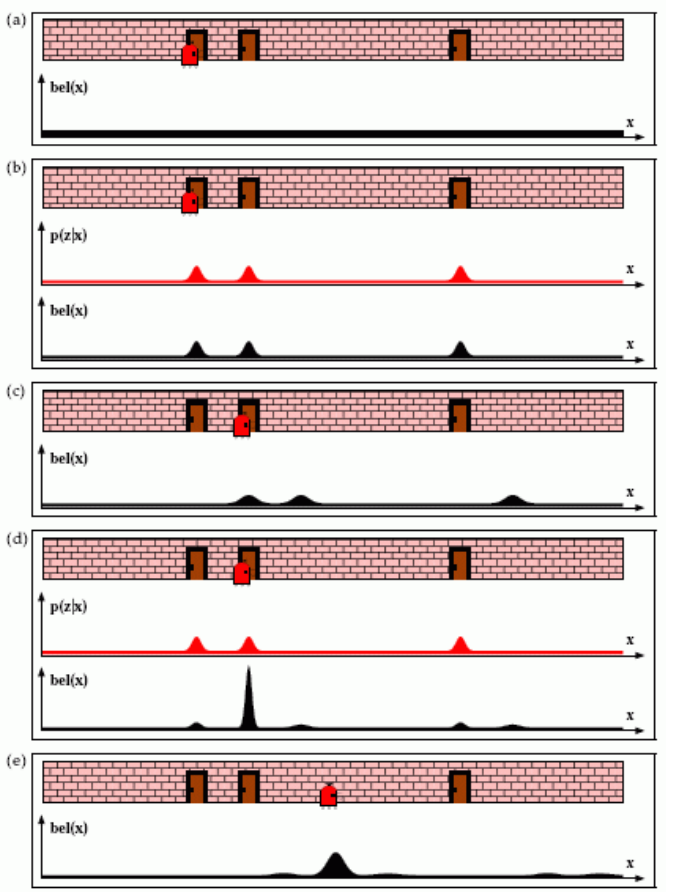
\includegraphics[scale=0.6]{Resources/PNG/MarkovAlgorithmus.PNG}
		\caption{}
		\label{fig:Resources/PNG/MarkovAlgorithmus.PNG}
	\end{center}
\end{figure}
\section{Monte Carlo Lokalisierung}
\subsection{Grundsätzliches Vorgehen}
\begin{itemize}
	\item Stichprobenbasierendes Approximationsverfahren
	\item Spezialform von Markov Lokalisierung
\end{itemize}
















